\section{System's Perspective}
\label{sec:systems_perspective}

\subsection{Overview}
\label{subsec:systems_perspective_overview}
The initial project was a full stack \textit{Flask} application written in \textit{Bash} and \textit{Python2} with an \textit{SQLite} database. 
This implementation (henceforth referenced as \mini) included refactoring the initial project to the following containerized microservices:
\begin{itemize}
    \item \textit{\cs}backend using the \textit{ASP.NET Core web framework} and \textit{EF Core} object-relational mapping.
    \item \textit{ReactJS} single-page application frontend.
    \item \textit{PostgreSQL} database.
\end{itemize}
Upon which a monitoring stack, and temporarily a logging stack, were added to be served as a containerized application behind a load-balancer on a managed \textit{Kubernetes} cluster (\textit{DOKS})

\subsection{System Design}
\label{subsec:system_design}
When we refactored the system we decided to change the architecture to follow The Clean Architecture guidelines, introduced by Robert C. Martin (reference here). We wanted the codebase to be easier to maintain, test and scale; and by that avoid technical debt.
We do this by following The Dependency Rule, which states that source code dependencies can only point inwards (reference here).

\begin{figure}[H]
    \centering
    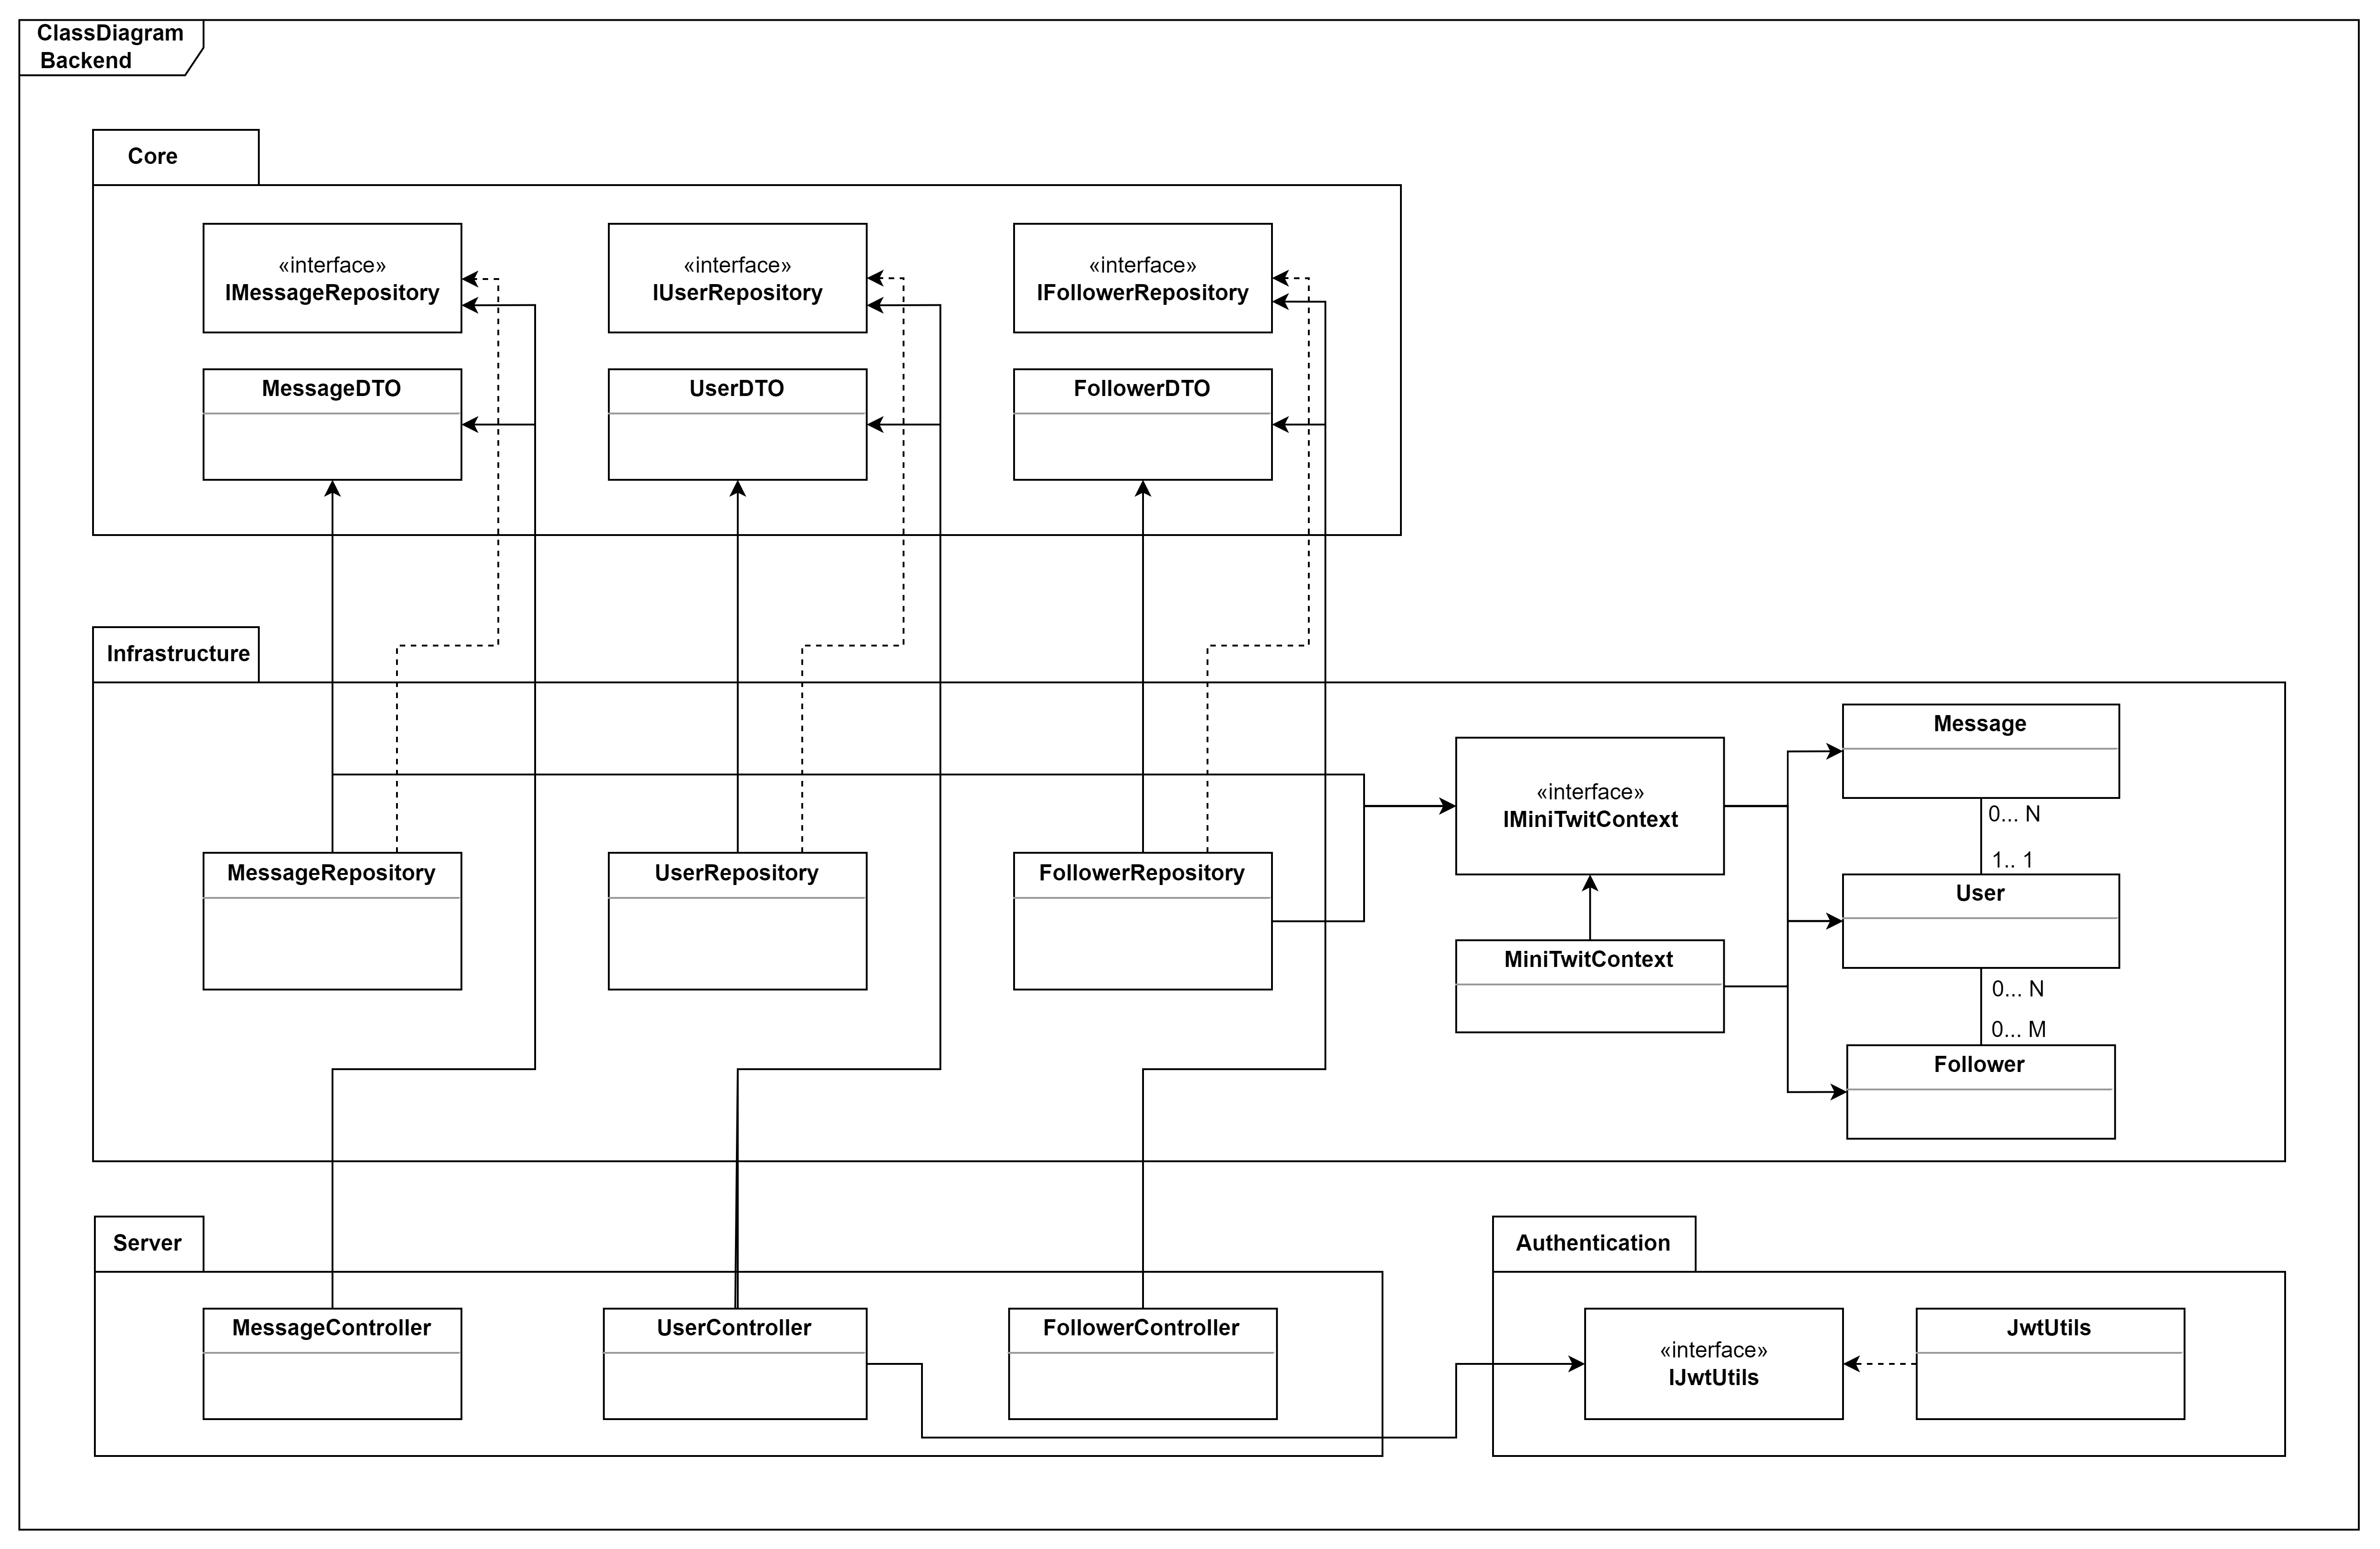
\includegraphics[scale=0.088]{images/package_class-diagrams/class_diagram_backend.png}
    \caption{Class Diagram Illustrating The Clean Architecture-pattern.}
    \label{fig:diagramClass}
\end{figure}

In figure \ref{fig:diagramClass} we can see the new refactored design: all dependencies point towards the core-package and each higher-level tier only have dependencies towards a tier closer to the core.  Note that each entity has a separate implementation of the repository-, DTO- and controller-class; this complies to the single responsibility principle. Additionally we only depend on abstractions, i. e. the UserController depend on the IUserRepository, not directly on implementation of UserRepository. All these principles derive from the SOLID-principles (also introduced by Martin).\\


The most interesting part of the system is the backend, which decomposition can be seen in Figure \ref{fig:decompositionBackend}.
Some files has been excluded in this diagram to simplify it. 
These files include Dockerfiles, Appsettings files, the program.cs file which is the entry point of the system, and a legacy controller and its interface for the frontend, which is now only used in tests. 

\begin{figure}[H]
    \centering
    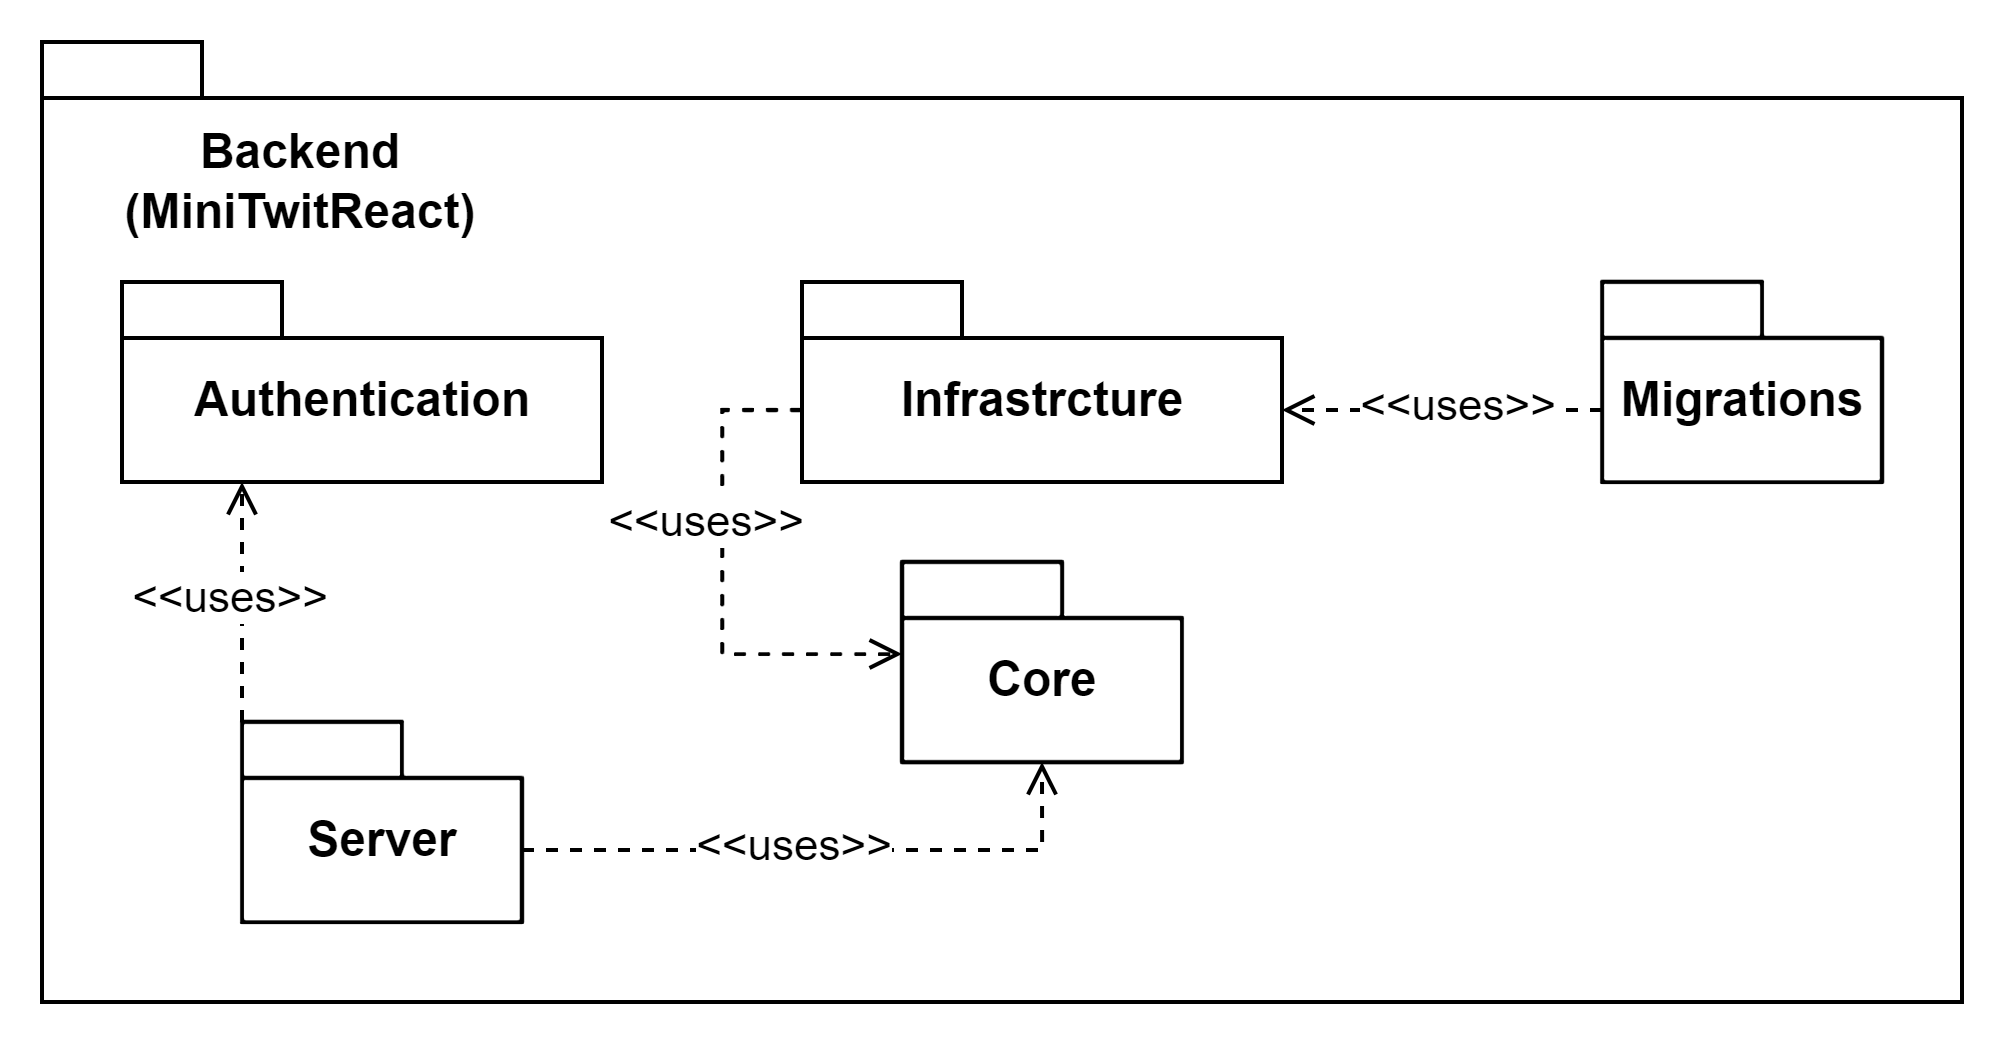
\includegraphics[scale=0.18]{images/package_class-diagrams/decomposition_backend.png}
    \caption{Decomposition of Backend Package of the \mini System}
    \label{fig:decompositionBackend}
\end{figure}


The system consists of 5 containerized microservices (see Figure \ref{fig:microservices}) of which the largest and most specific to our application is the \cs backend.
It contains the business logic, provides two open APIs, an Object-Relational Mapping to our database, and exposes application-specific \textit{PromQL} metrics for \textit{Prometheus}. \par

\begin{figure}[H]
    \centering
    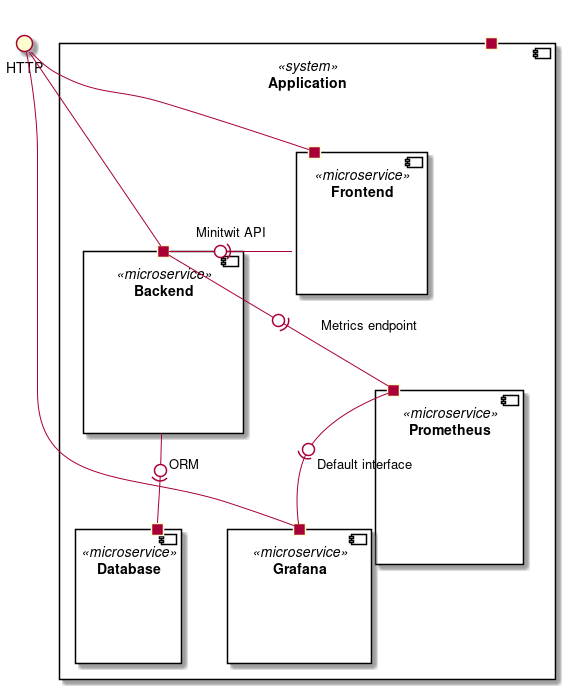
\includegraphics[scale=.43]{images/microservices-components.png}
    \caption{Component diagram of application microservices}
    \label{fig:microservices}
\end{figure}

This design pattern favors load balancing and horizontal scaling as most microservices serve a singular purpose and are non-critical to each other.

\subsection{System Architecture}
\label{subsec:system_architecture}
% - architecture of your itu-minitwit systems
% - all dependencies of your itu-minitwit systems on all levels of abstraction and development stages.
% - that is, list and briefly describe all technologies and tools you applied and depend on.
The \textit{Microservice Architecture} is achieved by separating the application into independently deployable parts. Figure \ref{fig:figdeployworker} illustrates how the backend, frontend, database, and monitoring stack are separated and run independently within individual containers. 
They communicate through the nodes' internal network and receive requests through the ingress controller proxy, which encrypts requests using an auto-renewed SSL certificate. 
persistent volumes are claimed through a persistent volume claim, see Figure \ref{fig:figdeployworker}, while secrets are retrieved by individual services from key-value storage, see  Figure \ref{fig:figdeploy}.

\begin{figure}[H]
    \centering
    \includegraphics[scale=0.43]{images/deployment_diagrams/devopsdiagrams-deployment worker nodes.drawio(3).png}
    \caption{\mini deployment diagram decomposition of worker nodes.}
    \label{fig:figdeployworker}
\end{figure}
The benefits of microservices are updating/deploying individual services, independently scaled services to support increased load, and integrating different stacks and programming languages, e.g., frontend, backend, and monitoring stack. However management and deployment complexity increases significantly when deploying services individually.\\
According to IBM, "\textit{Microservices both enable, and require, DevOps}", because this approach is unmanageable without implementing DevOps practices like automated CI/CD and monitoring\cite{microservices}.\\
Scaling and load balancing, is achieved by deploying services to a Kubernetes cluster on DigitalOcean, see scaling in section \ref{subsec:scaling}\\
%before - broken ref \hyperref[subsubsec:scalingprod]{2.7. scaling and load balancing}.
Kubernetes handles container orchestration to automate service discovery, networking, load balancing, rolling updates, and service health checking. Figure \ref{fig:figdeploy} visualizes the deployment of the \mini service on the cluster, showing the interaction between the worker nodes and the rest of the cluster.
\begin{figure}[H]
    \centering
    \includegraphics[scale=0.418]{images/deployment_diagrams/devopsdiagrams-deployment k8s.drawio(1).png}
    \caption{\mini deployment diagram}
    \label{fig:figdeploy}
\end{figure}
Through the Kubernetes command-line tool, \texttt{kubectl}, services can be deployed, updated, scaled, and inspected. The Load Balancer automatically distributes client requests to the proxies of different worker nodes.

\subsection{Technologies \& Tools}
\label{subsec:techs}
\mini depends on a number of different technologies and tools, dependencies from all development stages shown in Figure \ref{fig:dependencies}. 
\begin{figure}[H]
    \centering
    \includegraphics[scale=0.418]{}
    \caption{Technologies \& Tools on which \mini depend}
    \label{fig:dependencies}
\end{figure}


\subsection{Subsystem Interactions}
\label{subsec:subsystem_interactions}
% - important interactions of subsystems
\begin{figure}[H]
    \centering
    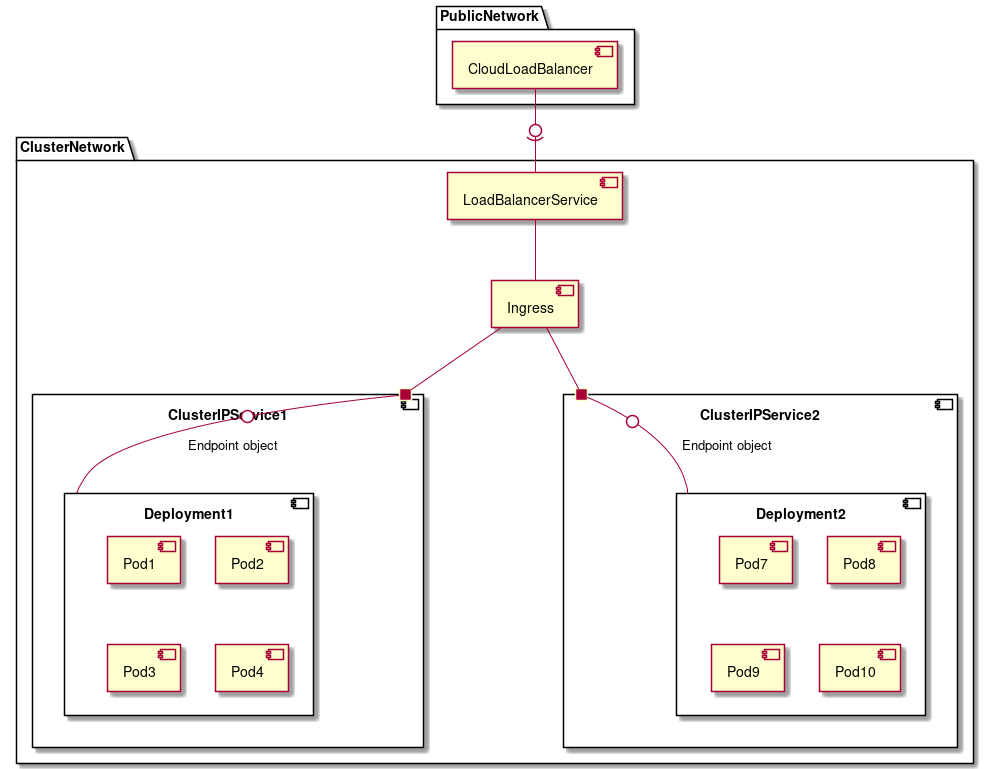
\includegraphics[scale=.4]{images/networking-class.png}
    \caption{Network Component Diagram}
    \label{fig:network_components}
\end{figure}
A notable downside of the microservice architectural pattern is the unreliability of networking interfaces, making IP tracking problematic when eliminating single points of failure and providing high availability to services.
\subsubsection{The Service Object}
The Kubernetes resource \texttt{Services}, provides stable IP addresses, DNS names, and ports through loose coupling to Deployments.
Traffic to microservices is sent to DNS addresses and resolved by the internal cluster DNS, to the IP address of the relevant Services, before being routed to healthy pods via an \texttt{Endpoint} object that stores a dynamic list of healthy pods matching the Service object's labels \cite{k8sbook}.

\subsubsection{The Cluster Network}
Kubernetes abstracts a cluster of hosts to a single platform, see \textit{Cluster Network} in Figure \ref{fig:network_components}, providing a filesystem, DNS, network, and memory sharing and computational resources. Any process or device connected is also discoverable on the network, allowing communication between pods give 
The Cluster Network operates similarly to a local network on any regular host in such a way that any device or process on the network is discoverable by other entities on the same network. 
Hence, given that a pod knows the IP of another pod on the cluster network, traffic between them is possible, though traffic via Service objects is preferable.
\subsubsection{The LoadBalancer}
The previously mentioned Service object has a few subtypes, including the \texttt{LoadBalancerService}, which is dependant on infrastructure.
When a Kubernetes LoadBalancerService is created, Kubernetes provisions a cloud load-balancer (see Figure \ref{fig:network_components}) via the cloud-platform in use, which is then interfaced by the LoadBalancerService. Note that LoadBalancers as all Service types can only interface one Deployment.
\subsubsection{The Ingress Object}
Ingress is all about accessing multiple web applications through a single Service object \cite{k8sbook}. 
Ingress is a Kubernetes resource which serves various purposes but most importantly provides a reverse proxy to multiple Service objects.

\subsection{System state}
\label{subsec:system_state}
% - Describe the current state of your systems, for example using results of static analysis and quality assessment systems.
% Wait until after cleanup when frontend is merged.
To be able to argue about the quality of our code, we have enhanced our \textit{CI} pipeline with static code analysis tools. These analyze and rate \mini per their definition of code quality.

\subsubsection{Code Quality, Technical Debt, \& Maintainability}
\label{subsubsec:code_quality}
\mini supports both a simulator API and an API for the frontend resulting in code duplication.\\
\textit{Sonarcloud} suggests that we have a technical debt of 55min, all of which is from the \texttt{Simulation Controller} and its infrastructure class, indicating that the simulation \texttt{controller} and \texttt{repository} requires refactoring. In contrast \textit{Code Climate}(see Appendix \hyperref[app:codeClimate]{A}) scores the technical debt of the system as 2 weeks and finds 17 code smells. This partly shows the difference in the definition of code quality between different tools. However, it is also caused by Code Climate analyzing the entire repository (see Appendix \hyperref[fig:codeClimateLangDis]{A}), while Sonarcloud analyzes only the backend (see Appendix \hyperref[fig:codeClimateLangDis]{A}). The frontend contributing heavily to technical debt was expected. Because of time constraints frontend code quality was not prioritized as highly as implementing weekly assignments and improving the backend. The difference in the definition of code quality of these tools is fascinating. \textit{DeepScan} at the same time detected no quality issues (see Appendix \hyperref[app:codeAnalDeep]{A}). \\
In conclusion, the technical debt of the frontend hurts the maintainability of the system. The backend has little to no technical debt, and code quality is good except for the simulation controller and simulation repository needing refactoring.

\subsubsection{Vulnerabilities}
2 dedicated security vulnerability scanning tools are used to increase chance of discovering vulnerabilities. Both \textit{Snyk}(see Appendix \hyperref[app:codeAnalSnyk]{A} and \textit{Dependabot}(see Appendix\hyperref[app:codeAnalDependabot]{A}) finds a vulnerability of high severity stemming from a \textit{npm} dependency, enforcing the fact that it is a known vulnerability. \\
In conclusion, the \mini code base contains two vulnerabilities in the frontend npm modules.


\subsection{License Compatibility}
\label{subsec:license_compatability}
% - Finally, describe briefly, if the license that you have chosen for your project is actually compatible with the licenses of all your direct dependencies.
%this is only a draft
The initial license chosen was \textit{MIT}, meaning everyone could use and modify the code freely.
However, when using \textit{ScanCode}\footnote{ScanCode Toolkit documentation\cite{Scancode}}, a tool to scan code for licenses, to determine if the license would clash with another license in the imports by scanning the files in the project. Through the result we discovered that some of our imports used \textit{Apache License 2.0}\footnote{Apache License 2.0 document\cite{Apache2.0}} and some packages \textit{BSD-3-Clause}\footnote{BSD-3-Clause\cite{BSD3Clause}}, meaning we had to change license.
The new license is Apache 2.0 as a result of running ScanCode to ensure the license is compatible. The scan seemed to fail on some licenses as it stated them as \textit{Unknown license}, however, since the other licenses encountered are the three mentioned previously, then it is likely not a problem. Additionally, when manually searching for the licenses on the imports we use in the frontend we discovered the majority used MIT license, and one used Apache license 2.0. Therefore the BSD-3-Clause might be some \textit{nodejs} dependency as the license is located in a few development packages alongside Apache license 2.0 and MIT license, but in none of used imports in the code.
%The backend had a license, \textit{IPA Font License} (copy left free font software license -- \textbf{ehh what does this mean?}), this is located in unit test, \textit{xunit}, related \texttt{.dll} files in our \texttt{integration tests} folder in a \texttt{bin/debug} folder. However since this license is only located in the unittests, however since our system is already free this license should not be a problem?
%this IPA Font seems to be something from Japan, idk how much we should include about it.

%Idk if you want to check for yourself if multiple licenses are used in the same file.. but an example is The pack in line 50432-51470 in result.json, which is quite a big file.

%React.router = mit license
%react-router-dom = mit license
%prop-types = mit license
%@mui/material = mit license
%markdown-to-jsx = mit license
%react = mit license
%react-router = mit license
%yup = mit license
%formik = Apache license 2.0

% A description and illustration of the:
% - Double check that for all the weekly tasks (those listed in the schedule) you include the corresponding information.